% !TeX program = lualatex
% !TeX encoding = UTF-8
\documentclass[tikz,12pt]{standalone}
  \usepackage{fontspec} 
  \setmainfont{Cambria} 

\graphicspath{{../src/FYZ/img/}}
\begin{document}
\hyphenchar\font=-1
\begin{tikzpicture}
    \node[anchor=south west,inner sep=0] 
        at (0,0) {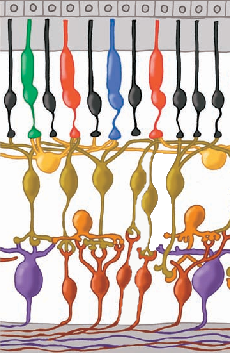
\includegraphics[width=\textwidth]{fyz_fig919.png}};
    \draw[black,ultra thick,->] (-1,20.0) node[left, text width=2.0cm]{pigment epithelium} -- (0,20);
    \draw[black,ultra thick,->] (-1,17.3) node[left, text width=2.0cm]{rods \emph{tyčinky}} -- (0.5,17.3);
    \draw[black,ultra thick,->] (-1,16) node[left, text width=2.0cm]{cones \emph{čípky}} -- (1.3,16);
    \draw[black,ultra thick] (-1,12)  node[left, text width=2cm]{outer plexiform layer} 
        -- (-.2,12)-- ++(0,.7cm) -- ++(.3cm,0) ++ (0,-1.4cm) -- ++ (-.3cm,0) -- ++ (0,0.7cm);
    \draw[black,ultra thick,->] (-1,10.5)  node[left, text width=2cm]{horizontal cells} -- (2.3,11.2);
    \draw[black,ultra thick,->] (-1,9.0)  node[left, text width=2cm]{bipolar cells} -- (1.4,10);
    \draw[black,ultra thick,->] (-1,7.5)  node[left, text width=2cm]{amarcrine cells} -- (4.4,8);
    \draw[black,ultra thick] (-1,6)  node[left, text width=2cm]{inner plexiform layer} %
        -- (-0.2,6) -- ++(0,.7cm) -- ++(.3cm,0) ++ (0,-1.4cm) -- ++ (-.3cm,0) -- ++ (0,0.7cm);
    \draw[black,ultra thick,->] (-1,3)  node[left, text width=2cm]{ganglion cells} -- (0.9,4);
    \draw[black,ultra thick,->] (-1,0.5)  node[left, text width=2cm]{nerve fiber layer} -- (0.05,0.5);
\end{tikzpicture}
\end{document}